% 生成最终的图象时把第一个文档类取消注释即可
\documentclass[10pt,varwidth]{standalone}
% \documentclass[12pt]{article}
% 1.必须添加varwidth选项,不然就会报错
\PassOptionsToPackage{quiet}{fontspec}
\usepackage{ctex}
% 必须要保证绘图的纸张足够的大
\usepackage[a4paper, left=2.5cm, right=2cm, top=2.5cm, bottom=2.5cm]{geometry}
\usepackage{xifthen}
\usepackage{xfp}
\usepackage{xcolor}
\usepackage{pgfplots}
\usepackage{pgfplotstable}
\pgfplotsset{compat=1.16}
% 2.引用的tikz库
\usetikzlibrary {matrix, chains, trees, decorations}
\usetikzlibrary {arrows.meta, automata,positioning}
\usetikzlibrary {decorations.pathmorphing, calc}
\usetikzlibrary {calligraphy}
\usetikzlibrary {backgrounds, mindmap,shadows}
\usetikzlibrary {patterns, quotes, 3d, shadows}
\usetikzlibrary {graphs, fadings, scopes}
\usetikzlibrary {arrows, shapes.geometric}
\usepgflibrary {shadings}



\begin{document}
\;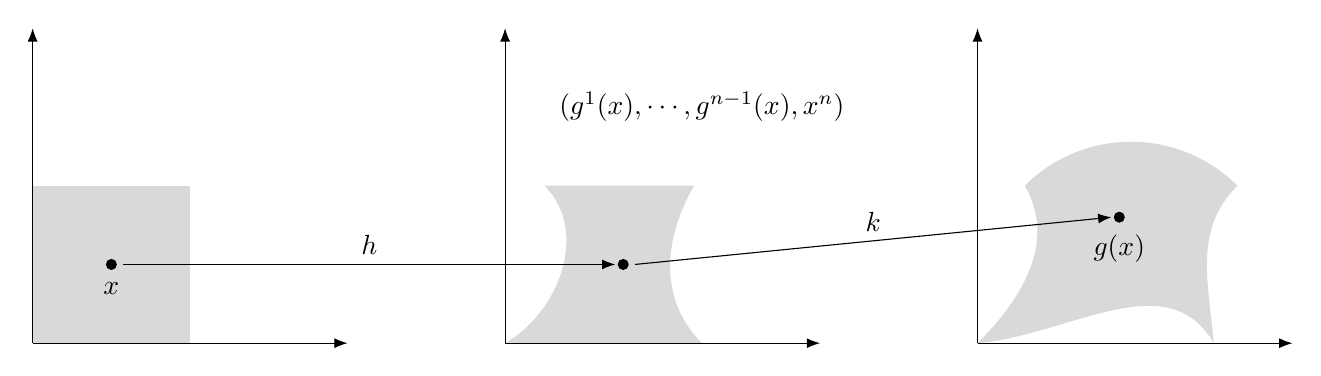
\begin{tikzpicture}[>=Latex]
    % out 和 in 分别对应出发点的 out 和目的点的 in
    \begin{scope}
        \fill[gray!30] (0, 0) rectangle (2, 2);
        \draw[->] (0, 0) -- (4, 0);
        \draw[->] (0, 0) -- (0, 4);
        \node (A) at (1, .7) {$x$};
        \fill (1, 1) circle (2pt);
    \end{scope}
    \begin{scope}[xshift=6cm]
        \fill[gray!30] (0, 0) -- (2.5, 0) to[out=135, in=-120] (2.4, 2) -- (.5, 2) to[out=-45, in=30] (0, 0);
        \draw[->] (0, 0) -- (4, 0);
        \draw[->] (0, 0) -- (0, 4);
        \node (A) at (2.5, 3) {$(g^1(x),\cdots,g^{n-1}(x),x^n)$};
        \fill (1.5, 1) circle (2pt);
    \end{scope}
    \begin{scope}[xshift=12cm]
        \fill[gray!30] (0, 0) 
            to[out=5, in=120]   (3, 0)
            to[out=95, in=-135] (3.3, 2)
            to[out=135, in=45]  (.6, 2)
            to[out=-60, in=45]  (0, 0); 
        \draw[->] (0, 0) -- (4, 0);
        \draw[->] (0, 0) -- (0, 4);
        \node (A) at (1.8, 1.2) {$g(x)$};
        \fill (1.8, 1.6) circle (2pt);
    \end{scope}
    % cross line
    \draw[->] (1.15, 1) -- (7.4, 1) node[midway, above] {$h$};
    \draw[->] (7.65, 1) -- (13.7, 1.6) node[midway, above] {$k$};
\end{tikzpicture}\;
\end{document}